
In this exercise we will get to know the programming tool Node-RED which will be used 
for wiring together hardware devices, APIs and online services in new and interesting ways.

As the tool is primary picture based, there will not be much code in this exercise.
The exported \code{.json} of the Node-RED flow can be found in the sheet 2 folder of the 
\url{https://github.com/Smokey95/AIN_Ubiquitous_Computing} in the exercise section.


\section{Exercise 1; Hello World}

We will start with an basic example to get familiar with the tool b< just triggering a 
simple \code{Hello World} message.

\begin{figure}[h!]
  \centering
  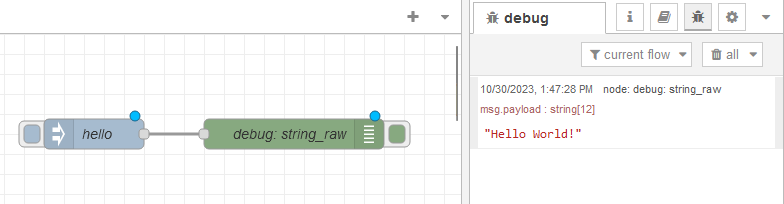
\includegraphics[width=1\textwidth]{exercise_node-red/exercise_1}
  \caption{Hello World}
  \label{fig:hello_world}
\end{figure}


\section{Exercise 2: Change Message}

In this exercise we will change the incoming \code{Hello World} message to \code{Hello Mars} and 
print it to the debug console.

\begin{figure}[h!]
  \centering
  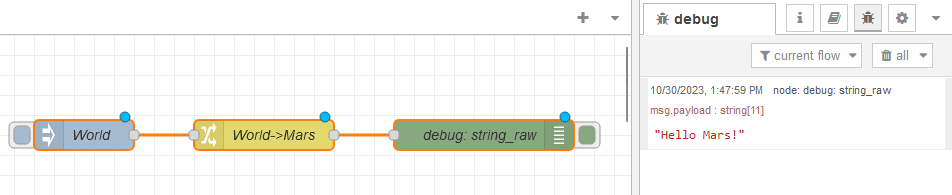
\includegraphics[width=1\textwidth]{exercise_node-red/exercise_2}
  \caption{Change Message}
  \label{fig:change_message}
\end{figure}


\section{Exercise 3: HTTP Request}

In this exercise we will use the \code{http request} node to get the current earthquake data from 
the \url{https://earthquake.usgs.gov/earthquakes/feed/v1.0/summary/significant_month.csv}.
It was decided to print the raw data to the debug console. Also the \code{change} node was used to 
change payload where the \code{mag} data was greater than 5.3 to \code{Panic!}.

\begin{figure}[h!]
  \centering
  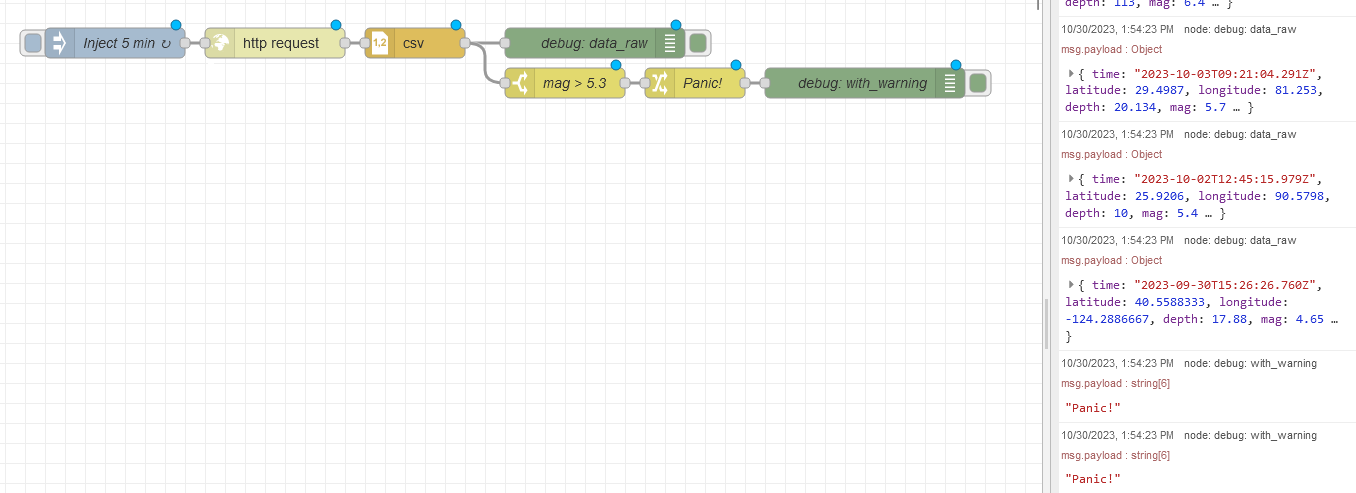
\includegraphics[width=1\textwidth]{exercise_node-red/exercise_3}
  \caption{HTTP Request}
  \label{fig:http_request}
\end{figure}


\section{Exercise 4: Dashboards}

In this exercise we will use the \code{dashboard} node to create a simple dashboard which will 
show the current time in several different formats.

\begin{figure}[H]
  \centering
  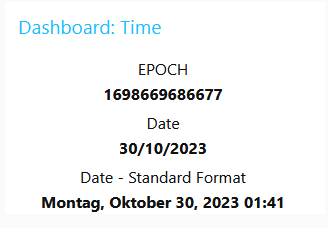
\includegraphics[width=0.8\textwidth]{exercise_node-red/exercise_4_dashboard}
  \caption{Dashboard}
  \label{fig:dashboard}
\end{figure}

\begin{figure}[H]
  \centering
  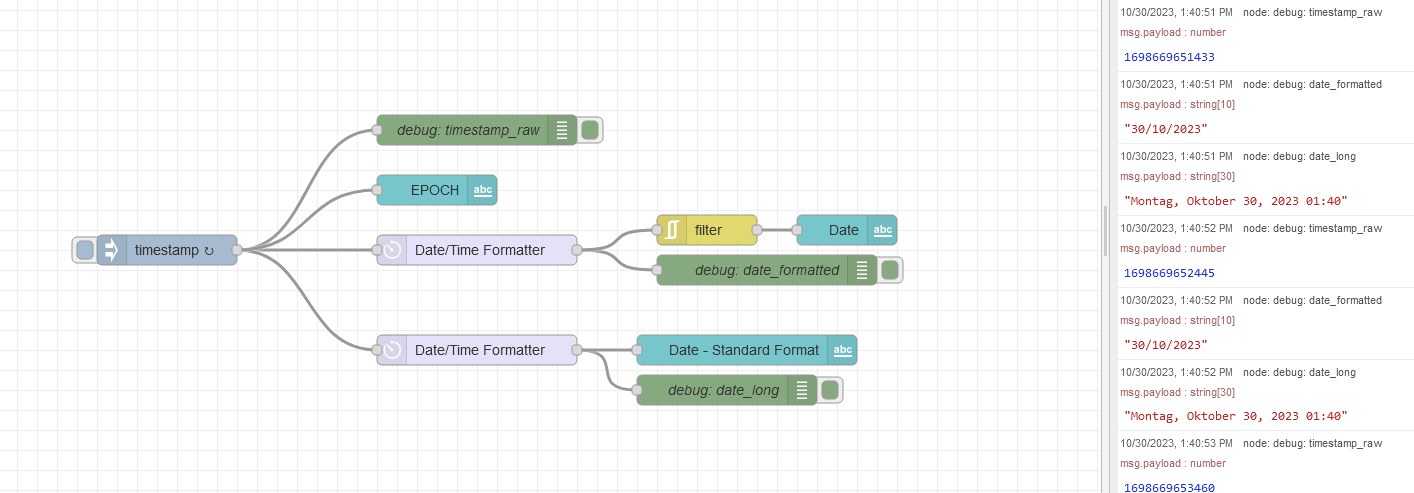
\includegraphics[width=1\textwidth]{exercise_node-red/exercise_4_node}
  \caption{Nodes}
  \label{fig:4_nodes}
\end{figure}

To display the date with written day name and month some time were spent to find the correct 
formatting of \code{dddd, MMMM DD, YYYY hh:mm} to display the timestamp like wanted.


\section{Exercise 5: LED Control}

%% under construction


\section{Exercise 6: Temperature}

In this exercise we will use the \code{gauge} node to display the current temperature of the 
Arduino board. The temperature is measured using the internal temperature sensor of the Arduino. 
It was not a requirement but i tried to reuse the code from the first exercise with no changes 
leading to expanded node red flow.

\begin{figure}[H]
  \centering
  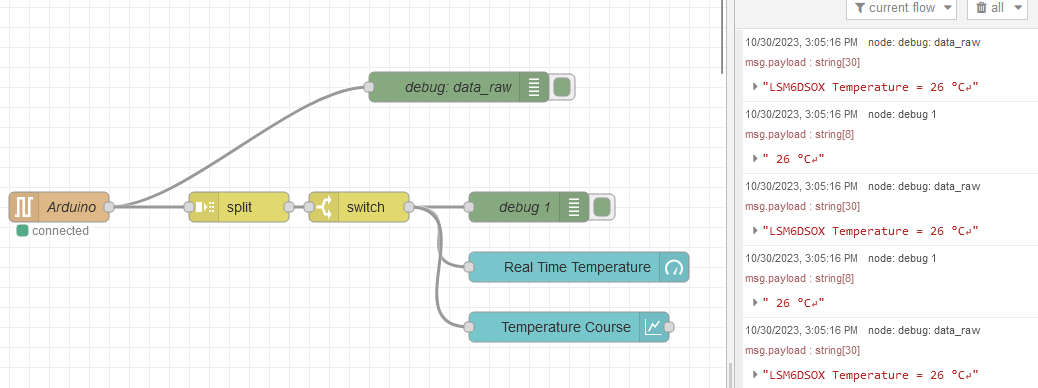
\includegraphics[width=1\textwidth]{exercise_node-red/exercise_6_full}
  \caption{Temperature}
  \label{fig:temperature}
\end{figure}

Like seen in the figure above, the Arduino board prints the current temperature to the serial port 
like in the code from the first exercise. To process this data the \code{split} node was used to 
split the incoming data stream and a \code{switch} node which will compare incoming data if it 
\code{contains °C} and only forward this data.

The resulting dashboard can be seen in the figure below.

\begin{figure}[H]
  \centering
  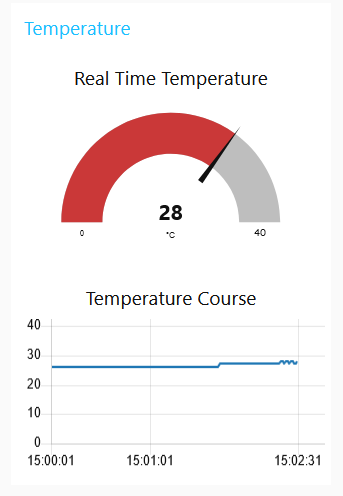
\includegraphics[width=1\textwidth]{exercise_node-red/exercise_6_dashboard}
  \caption{Temperature Dashboard}
  \label{fig:temperature_dashboard}
\end{figure}


\section{Exercise 7: MQTT}

In this exercise we will use the \code{mqtt} node to send the current temperature to a MQTT broker 
(hosted on \url{https://www.hivemq.com/try-out/}) and display it on a dashboard 
on \url{https://www.datacake.de/}.

Most effort was spent on this exercise cause it was not clearly described (or at least for me) 
how important the \code{topic} field is. This field has to match either in Node-RED config 
as well as on the datacake settings. Even after figure this out the data was not processed 
right so i created a second flow which send the data to the broker where it will be 
returned as \code{raw\_data}.

Also it has to be noted that this time the code of the Arduino was changed to send the 
temperature in a json styled format to the serial port. As most of the code was not changed 
only the relevant part is shown below.

\begin{minted}
  [
    frame=lines,
    framesep=2mm,
    baselinestretch=1.2,
    linenos
  ]
  {C}

  ...
  // Offset of ~30%
  float temperature_normalized = temperature_deg / 1.3;

  // Create a JSON-formatted string
  String jsonString = "{\"temp\": " + String(temperature_normalized) + "}";

  // Send JSON-formatted string over serial
  Serial.println(jsonString);
  ...

\end{minted}

This data will then rooted from the serial port to the \code{mqtt} node which will send it to 
the broker. Notice that the data will be send to two different topics. One topic is used to 
send data to an raw channel and the other one is used to send data to a formatted channel (see 
figure below).

\begin{figure}[H]
  \centering
  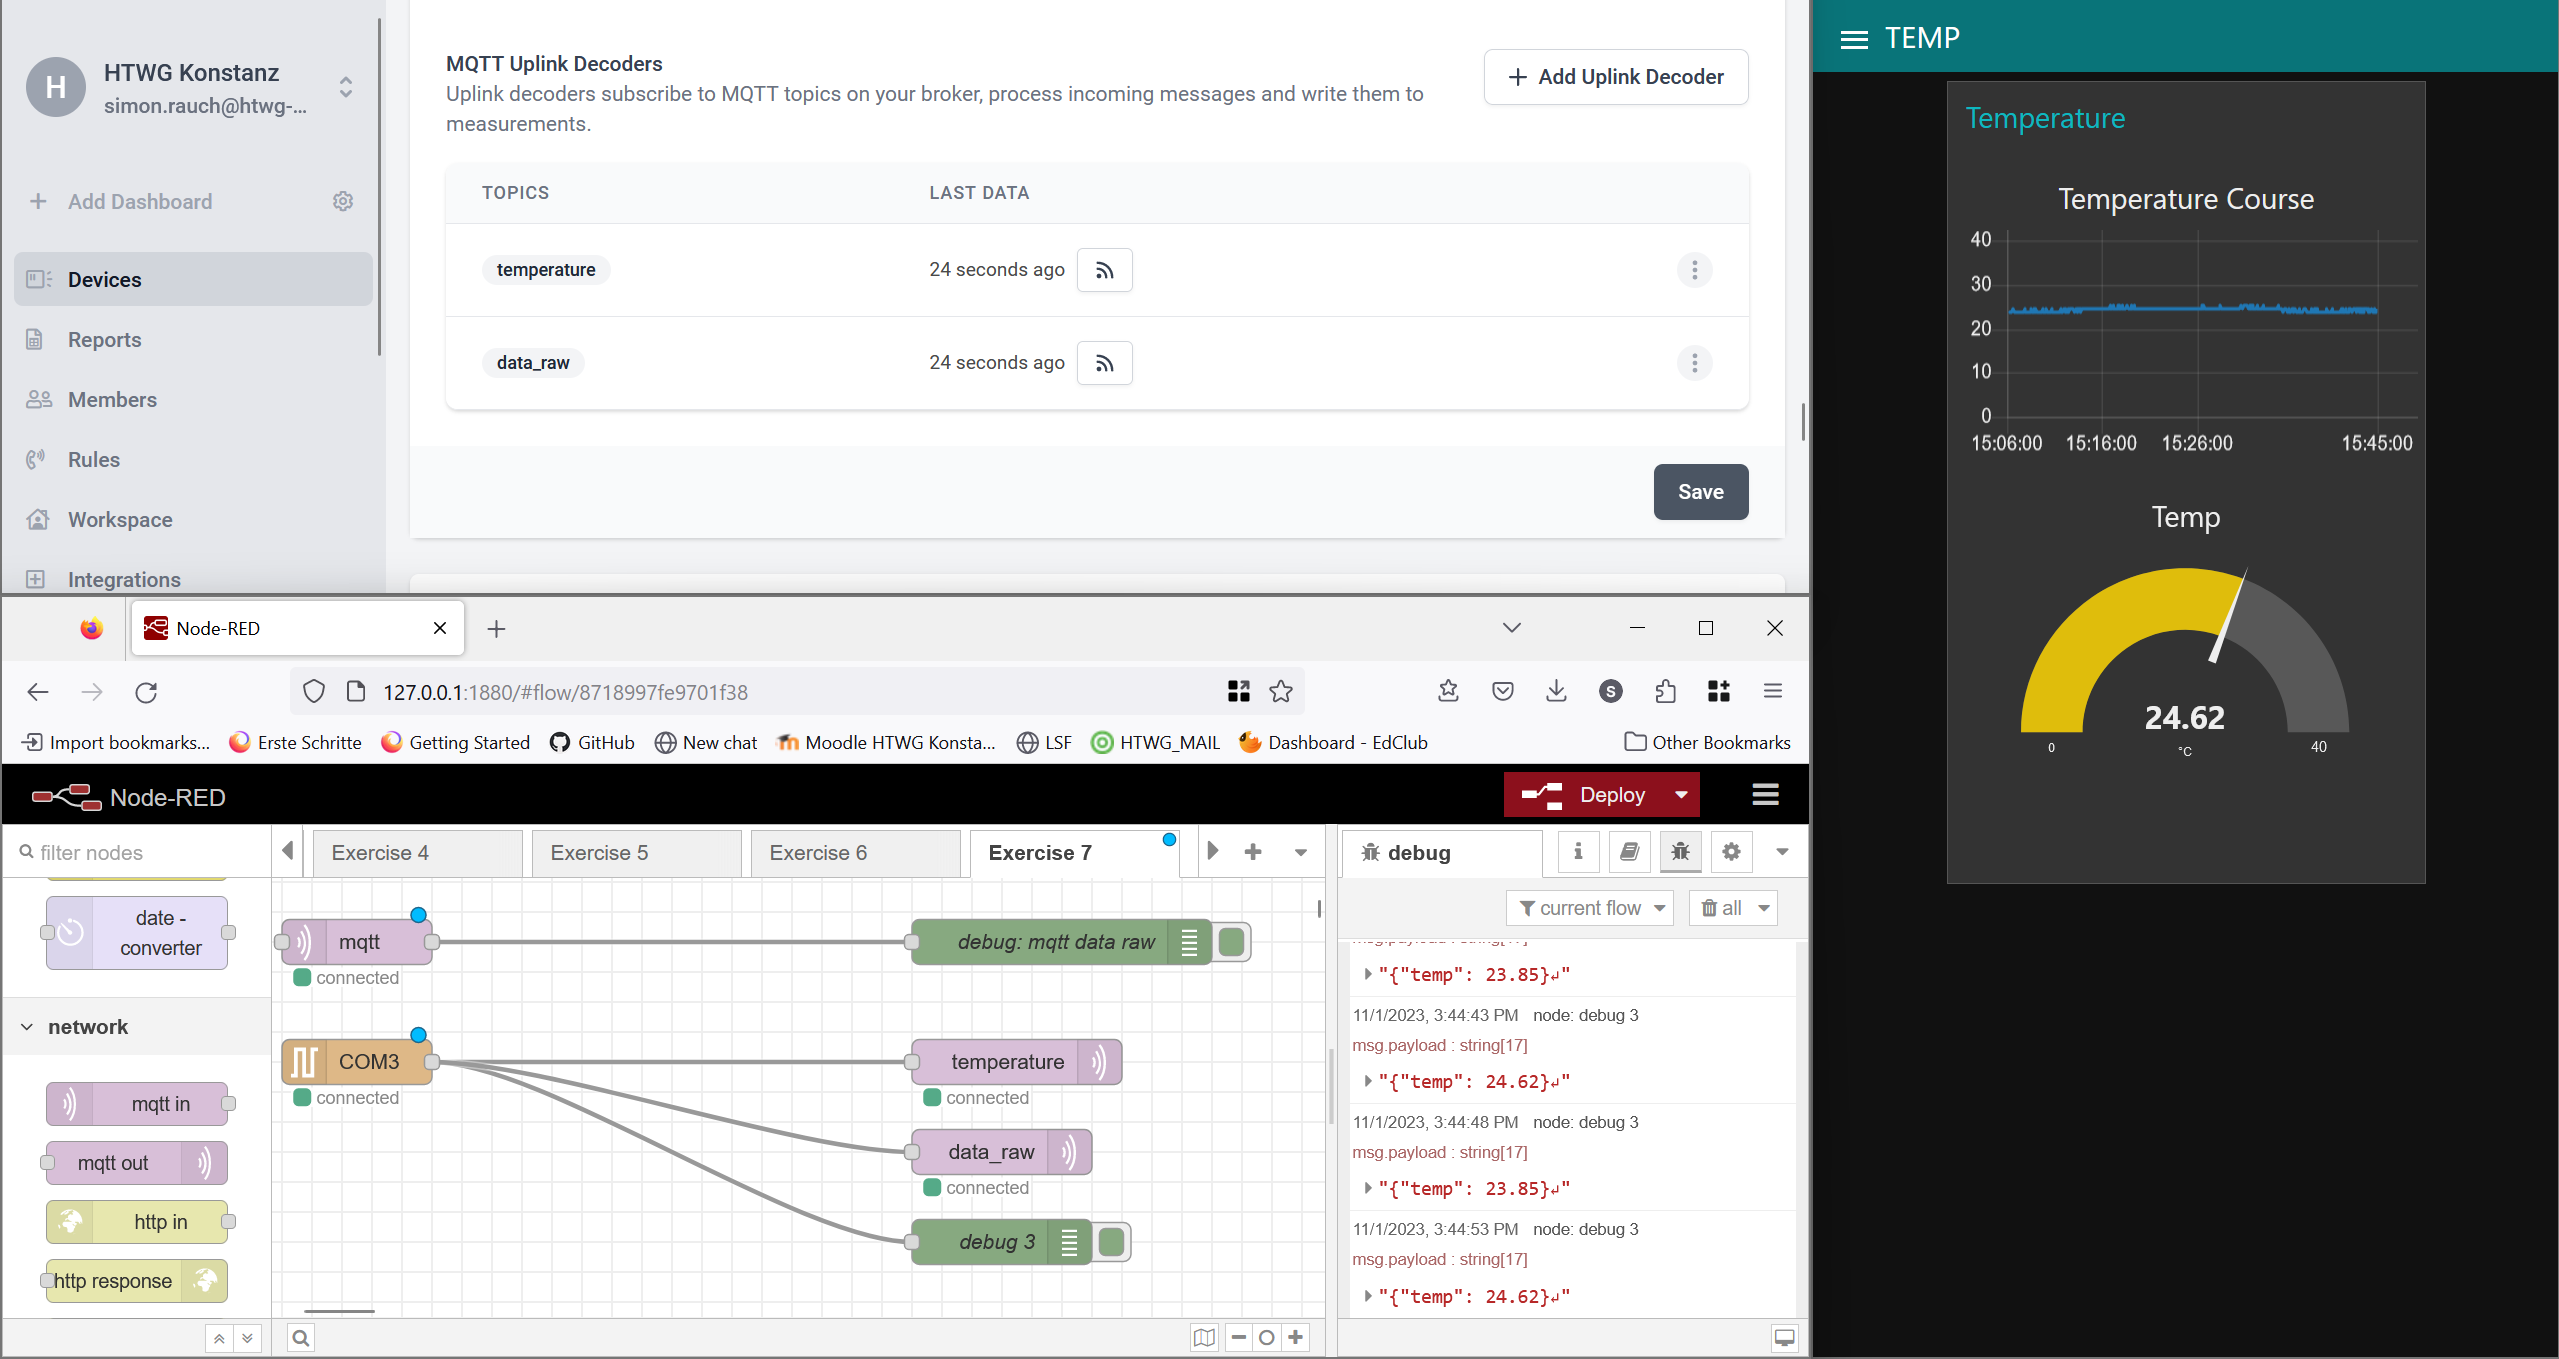
\includegraphics[width=1\textwidth]{exercise_node-red/exercise_7_data_raw}
  \caption{MQTT}
  \label{fig:mqtt}
\end{figure}

I spent some more time cause i does not why but even if the same data was send to both topics 
only the raw data was seen on datacake even if both Uplink decoder were the same. 
To waste no more time the decoder from the temperature channel was moved to the raw channel 
which worked fine and data was displayed on the dashboard.
Following you will see the java script to parse the data from the raw channel to the temperature field 
as well as the dashboard.

\begin{minted}
  [
    frame=lines,
    framesep=2mm,
    baselinestretch=1.2,
    linenos
  ]
  {javascript}

  function Decoder(topic, payload) {
    // Transform incoming payload to JSON
    payload = JSON.parse(payload);
    
    // Extract Temperature from payload, do calculation
    var temperature = payload.temp;
    
    // Forward Data to Datacake Device API using Serial, Field-Identifier
    return [
        {
            device: "e8aec33d-a641-4d25-a235-786fd1291a7b", // Serial Number or Device ID
            field: "TEMPERATURE",
            value: temperature
        },
    ];
  }
\end{minted}

\begin{figure}[H]
  \centering
  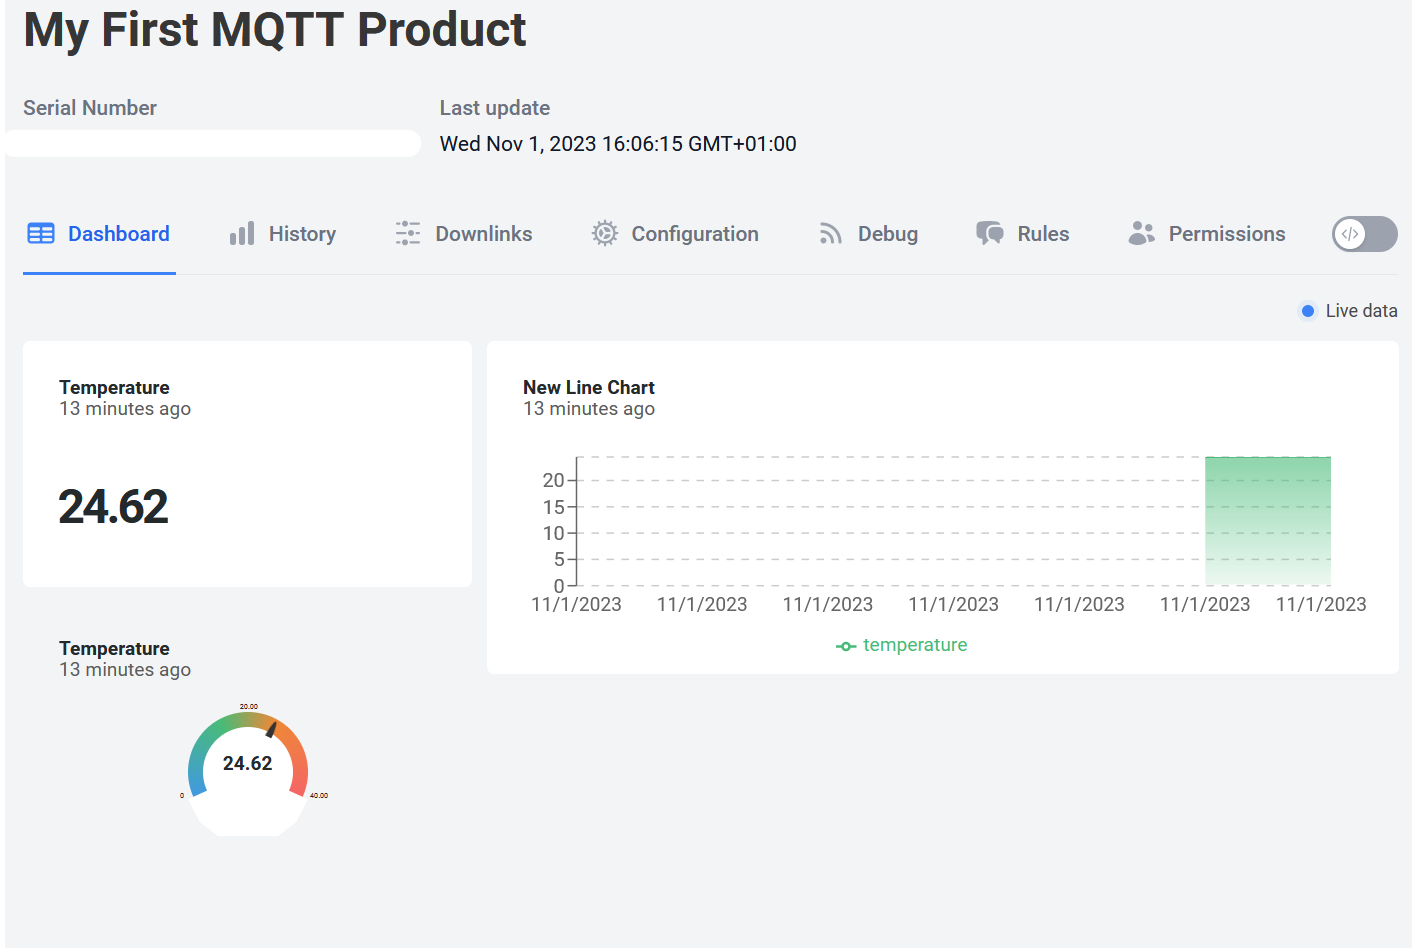
\includegraphics[width=0.8\textwidth]{exercise_node-red/exercise_7_dashboard}
  \caption{MQTT Dashboard}
  \label{fig:mqtt_dashboard}
\end{figure}

At the end of this exercise a downlink was setup to send a message to the Arduino board.
This was also a little bit frustrating but the config as well as the result can be seen below.

\begin{figure}[H]
  \centering
  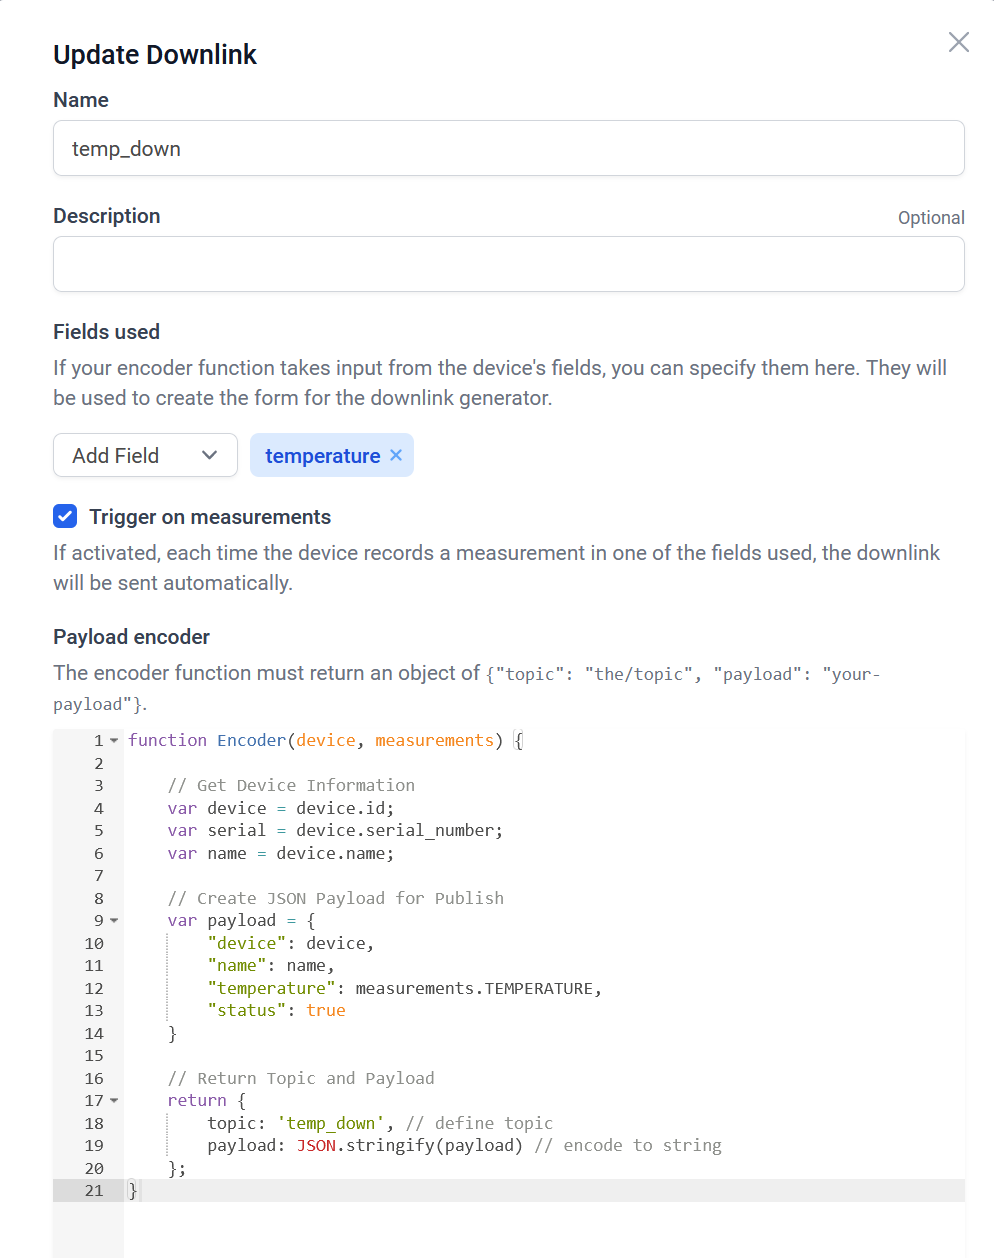
\includegraphics[width=0.8\textwidth]{exercise_node-red/exercise_7_downlink}
  \caption{MQTT Downlink}
  \label{fig:mqtt_downlink}
\end{figure}

\begin{figure}[H]
  \centering
  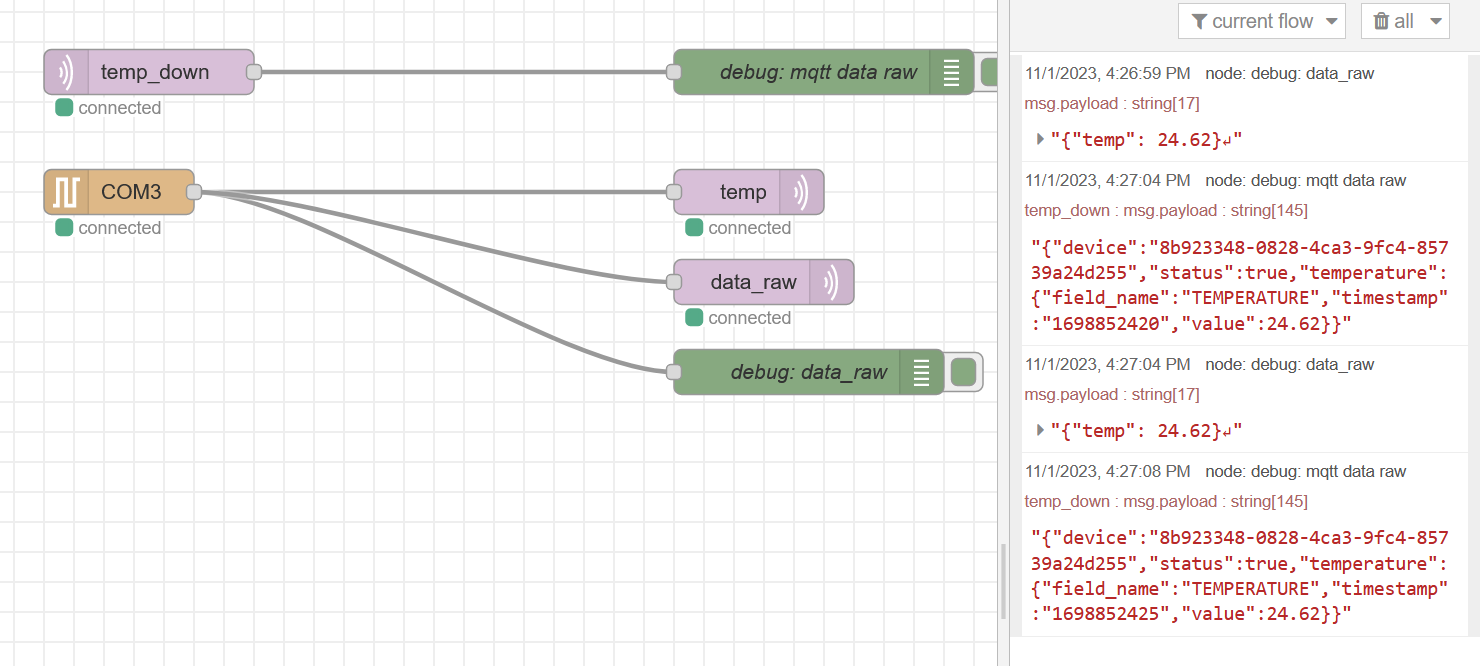
\includegraphics[width=0.8\textwidth]{exercise_node-red/exercise_7_data_down}
  \caption{MQTT Downlink Result}
  \label{fig:exercise_7_data_down}
\end{figure}